
\begin{figure}
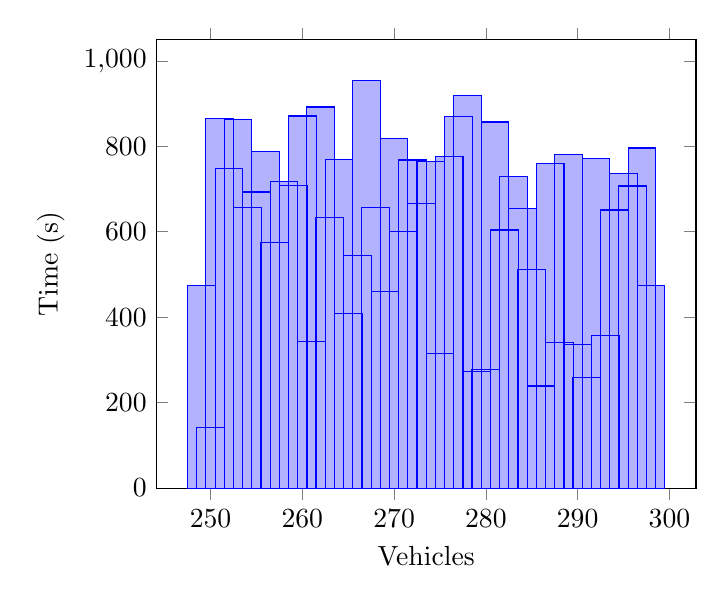
\begin{tikzpicture}
\begin{axis}[
legend style={anchor=west},
xlabel=Vehicles,
ylabel=Time (s),
ymin=0,
ybar,
]
\addplot coordinates {
(263, 634)
(286, 239)
(288, 341)
(295, 737)
(261, 343)
(282, 604)
(292, 772)
(275, 315)
(278, 918)
(255, 693)
(291, 259)
(289, 781)
(267, 954)
(298, 475)
(279, 273)
(260, 871)
(258, 718)
(297, 796)
(273, 666)
(251, 865)
(296, 707)
(283, 730)
(269, 461)
(284, 654)
(262, 892)
(252, 748)
(268, 656)
(254, 656)
(266, 544)
(271, 600)
(259, 709)
(257, 575)
(281, 857)
(265, 409)
(290, 336)
(270, 818)
(250, 141)
(272, 768)
(277, 869)
(293, 358)
(256, 787)
(280, 277)
(285, 512)
(249, 475)
(264, 769)
(287, 759)
(276, 777)
(274, 764)
(253, 863)
(294, 651)
};

\end{axis}
\end{tikzpicture}
\label{tik:time:100:90}
\caption{100 percent diving with GSC on route $90$}
\end{figure}
